Tässä luvussa ...

\begin{figure}[ht!]
  \centering
  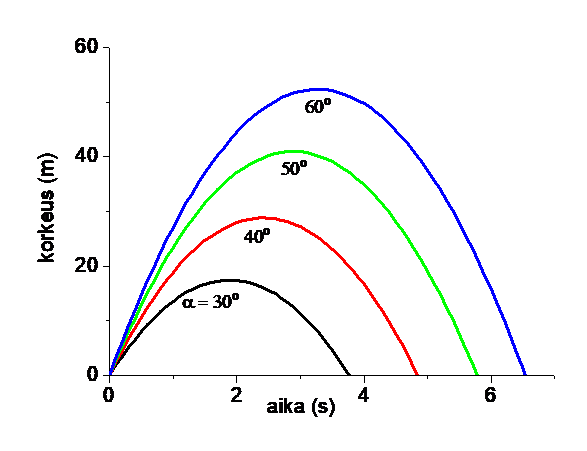
\includegraphics[width=0.5\textwidth]{assets/good-example.png}
  \caption{<Lisää kuvateksti tähän.>}
  \label{fig:kuvaesimerkki}
\end{figure}

\begin{table}[ht!]
  \centering
  \caption{<Lisää taulukkoteksti tähän.>}
  \label{tab:taulukkoesimerkki}
  \begin{tabular}{p{0.2\linewidth} | p{0.3\linewidth} | p{0.3\linewidth}}
    \hline
    & \textbf{Otsikko 1} & \textbf{Otsikko 2} \\
    \hline
    \textbf{Otsikko 3} & Teksti 1 & Teksti 2\\
    \hline
    \textbf{Otsikko 4} & Teksti 3 & Teksti 4\\
    \hline
  \end{tabular}
\end{table}

\parencite{nawar_multi-heuristic_2014}

\parencite{zhang_test_2007}